\documentclass[UTF8]{ctexart}
\usepackage{amsmath}
\usepackage{amsfonts}
\usepackage{amssymb}
\usepackage{graphicx}
\usepackage{hyperref}
\usepackage{float}
\usepackage{caption}
\usepackage{subfig}
\usepackage{bm}
\usepackage{mathrsfs}
\usepackage{latexsym}
\usepackage{euscript}
\usepackage{esint}
\usepackage{blindtext}
\usepackage{multirow}
\renewcommand\thesection{\Roman{section}}

\hypersetup{colorlinks=true,linkcolor=black}

% Title Page
\title{$ \alpha $ 粒子测量实验报告}
\author{17377306\ 马晓天}
\RequirePackage[a4paper]{geometry}
\geometry{
	textwidth=138mm,
	textheight=215mm,
	left=27mm,
	right=27mm,
	top=25.4mm, 
	bottom=25.4mm,
	headheight=2.17cm,
	headsep=4mm,
	footskip=12mm,
	heightrounded,
}


\begin{document}
\maketitle

\thispagestyle{empty}
\section{数据分析}
实验条件为：$^{241}$Am放射源(源号16AM4R5028，尺寸$ \Phi35\times1\rm mm $，发射率$\rm 1.51\times10^{6}/2\pi\cdot min^{-1} $)，金硅面垒半导体探测器(型号未记录)，低压电源为12V，偏压电源为60V(测量能谱时)，放大器放大倍数为$ 0.850\times50=42.5 $，成形时间1$ \mu $s，道数为16384。
实验原始数据为:
\begin{table}[H]
	\centering
	\caption{5V偏压下能量分辨率与成形时间表}
	\begin{tabular}{cccc}
		\hline
		成形时间/$ \mu $s & FWHM & CH & $ \eta $ \\
		\hline
		0.5&75.77&8191.92&0.009249\\
		1&63.73&8559.94&0.007445\\
		2&126.61&8852.85&0.014302\\
		3&74.92&8783.00&0.008530\\
		6&109.42&8656.34&0.012640\\
		10&101.67&8809.26&0.011541\\
		\hline
	\end{tabular}
\end{table}
其中，CH是峰值对应道址，FWHM是峰的半高宽，$ \eta $是能量分辨率。由能量分辨率可确定最佳成形时间为在1$ \mu $s，在 1$ \mu $s成形时间下改变偏压，得到以下数据：
\begin{table}[H]
	\centering
	\caption{1$ \mu $s成形时间下能量分辨率与偏压表}
	\begin{tabular}{ccccc}
		\hline
		偏压/V & 漏电流/$ \mu $A & FWHM & CH & $ \eta $ \\
		\hline
		5&0.04&63.73&8559.94&0.007445\\
		10&0.09&67.65&8894.99&0.007605\\
		30&0.22&73.57&8979.31&0.008286\\
		60&0.36&81.53&8999.69&0.009059\\
		100&0.52&103.43&9006.33&0.011484\\
		150&0.70&114.59&9007.61&0.012721\\
		\hline
	\end{tabular}
\end{table}
由能量分辨率可确定最佳偏压为5V，实验中采用偏压为60V，推测误差较大原因为CH和FW\\HM的测量误差。

\subsection{抽真空与不抽真空条件下输出波形的变化}
不抽真空条件下输出波形为无，抽真空之后输出波形如图1：
\begin{figure}[H]
	\centering
	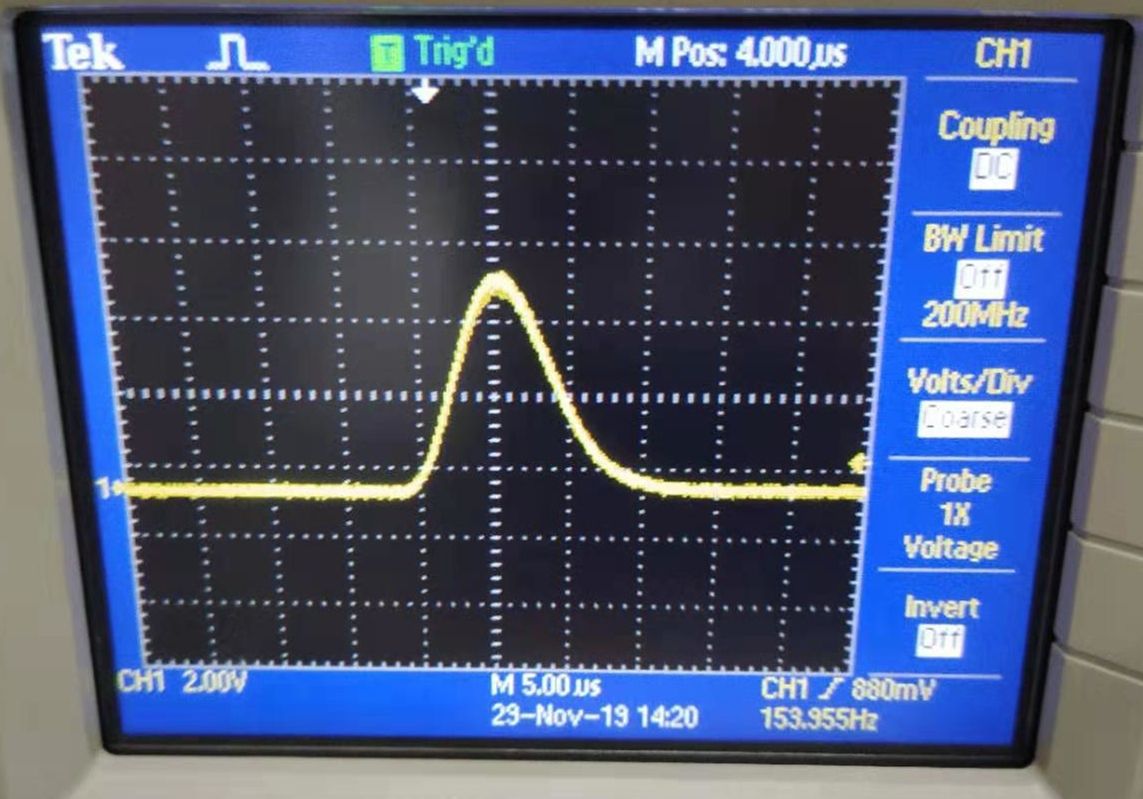
\includegraphics[width=0.6\linewidth]{bo.jpg}
	\caption{真空条件下输出波形图}
\end{figure}

\subsection{测量薄箔样品的能谱与待测薄箔样品的厚度计算}
$ \alpha $粒子的吸收峰为高斯峰，采用如下函数族进行拟合：
\begin{equation}
y=y_{0}+\frac{A}{w \sqrt{\pi / 2}} e^{-2 \frac{\left(x-x_{\mathrm{c}}\right)^{2}}{w^{2}}}
\end{equation}
通过高斯拟合可得，三组实验峰位：
\begin{equation*}
x_{c_{1}}=8985.74\pm0.55,\chi^{2}=226.7144,R^{2}=0.9675
\end{equation*}
\begin{equation*}
x_{c_{2}}=8541.36\pm0.65,\chi^{2}=146.9483,R^{2}=0.9644
\end{equation*}
\begin{equation*}
x_{c_{3}}=7541.58\pm0.76,\chi^{2}=87.5465,R^{2}=0.9618
\end{equation*}
由此可得三组已知厚度的$\alpha$粒子的吸收峰的峰位(道址)为(从左到右分别为不放铝箔、放置2$ \mu $m和\\6$ \mu $m铝箔的吸收峰)如下，拟合效果如图2。
\begin{equation}\label{key}
x_{\rm p_{1}}=x_{c_{1}}=8985.74\pm0.55,x_{\rm p_{2}}=x_{c_{2}}=8541.36\pm0.65,x_{\rm p_{3}}=x_{c_{3}}=7541.58\pm0.76
\end{equation}
查阅衰变纲图可得，未放置铝箔时$\alpha$粒子能量为5.486MeV，再由已知的数据$ E(x_{\rm p_{2}})=5.168\mathrm{MeV},\\E(x_{\rm p_{3}})=4.495\rm MeV $，由此可拟合出能量道址关系式为：
\begin{equation}
E=(0.684\pm0.010)x_{\rm p}-(666\pm83)(\rm kev)
\end{equation}
能量在1keV-10MeV之间的$ \alpha $粒子在铝中的阻止本领S，可用经验公式表示为：
\begin{equation}\label{key}
S=N\cdot\frac{A_{1} E A_{2}\left\{\frac{A_{3}}{E / 1000} \ln \left[1+\frac{A_{4}}{E / 1000}+\frac{A_{5} E}{1000}\right]\right\}}{A_{1} E A_{2}+\frac{A_{3}}{E / 1000} \ln \left[1+\frac{A_{4}}{E / 1000}+\frac{A_{5} E}{1000}\right]}
\end{equation}
其中，$ E$的单位为keV，铝原子数密度$N=7.714\times10^{22}\rm Atom/ cm^{3} $，$ (A_{1},A_{2},A_{3},A_{4},A_{5})=$ (2.5,\\0.625, 45.7, 0.1, 4.359)，代入$ E=5.486 $MeV可得对应能量的阻止本领$ S=2.060\times10^6\rm keV/cm $。
\begin{figure}[H]
	\centering
	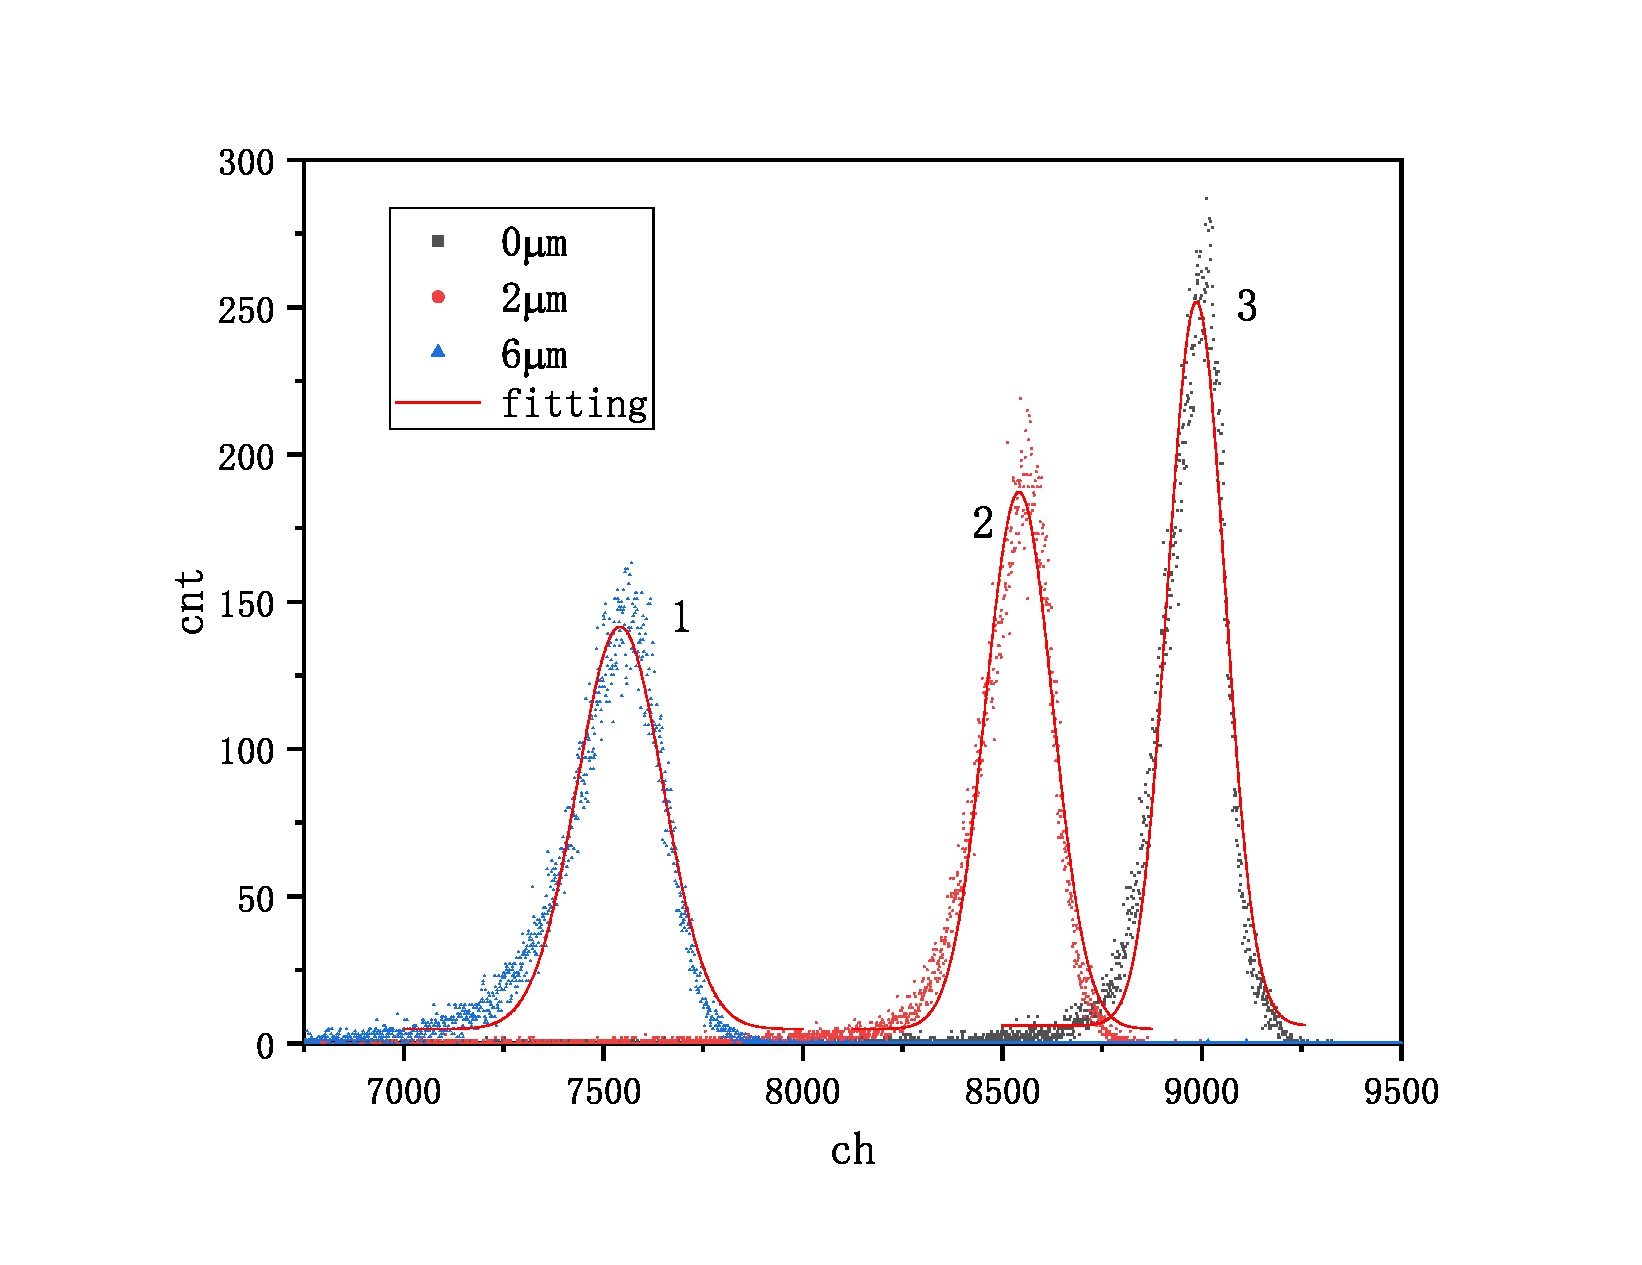
\includegraphics[width=0.9\linewidth]{alpha.eps}
	\caption{$ \alpha $粒子能谱图}
\end{figure}
当能量为$ E_{1} $的带电粒子，穿过厚度为$ \Delta x$的吸收体后，能量变化$ \Delta E$可表示为：
\begin{equation}\label{key}
\Delta x = \sum_{E_{1}}^{E_{1}+\Delta E}\frac{\delta E}{S}
\end{equation}
由高斯拟合可得未知厚度的吸收峰的峰位(道址)为：
\begin{equation}
x_{\rm p_{4}}=x_{c_{4}}=8467.67\pm0.87,\chi^{2}=77.4422,R^{2}=0.9571
\end{equation}
相应的能量$ E(x_{\rm p_4})=(5126\pm119)\rm keV $，代入式(5)，取$ \delta E=10\rm keV $可求得未知厚度：
\begin{equation}\label{key}
\Delta x=1.706_{-0.560}^{+0.551}\rm \mu m
\end{equation}

\section{误差分析}
未知厚度标定值是2$ \mu $m，相对误差=$-14.7_{-28.0}^{+27.6}\% $。推测误差主要原因为：(1)探头前的金属片对$ \alpha $粒子有吸收；(2)拟合时高斯峰左半边有拖尾使拟合带来误差，这也使得定标的精度误差较大；(3)探头有一定的面积。

\newpage
\section{思考题}
\paragraph{1.解释脉冲幅度和分辨率随偏压变化曲线的特征，并说明选择探测器偏压应考虑哪些因素？}
(1)能量分辨率随偏压先变小后变大，因为偏压越高产生的电子空穴对越多，但是漏电流也会增加使得噪声变大，因而呈现先变小后变大的趋势。
(2)应考虑尽量高的能量分辨率和合适的漏电流。

\paragraph{2.定性讨论$ \alpha $粒子穿过吸收体后能谱展宽的原因。}
放射源放出的$ \alpha $粒子能量分布有一定的展宽以及在半导体中产生电子空穴对的数目有一定涨落。

\section{实验总结}
本次实验使用半导体$\alpha$谱仪进行$ \alpha $粒子能谱的测定，探究了能量分辨率与成形时间和偏压的关系，了解$\alpha$粒子通过物质时的能量损失及其规律，掌握了相关的数据处理和分析方法，并且在数据处理和撰写实验报告中熟悉了对Origin和\LaTeX{}的使用，实验和数据处理能力大大提高。另外，老师理论课上讲的通过实践获得了更深的理解，掌握更牢。

\end{document}